\documentclass[14pt]{beamer}

\usepackage{xcolor}
\usepackage{colortbl}
\usepackage{pgf}
\usepackage{amsmath}
\usepackage{amssymb}
\usepackage{latexsym}
\usepackage{tikz}
\usepackage{pgfplots}
\usepackage{pdfpages}
\usepackage{ulem}

%\includeonlyframes{overview}

\usetikzlibrary{positioning, shapes}
\usetikzlibrary{decorations.pathmorphing}

\definecolor{shaded}{RGB}{210,210,210}
\usecolortheme[named=shaded]{structure}

\definecolor{stressed}{RGB}{150,40,40}
\setbeamercolor{alerted_text}{fg=stressed}


\setbeamertemplate{navigation symbols}{}
\setbeamersize{text margin left=3mm} 
\setbeamersize{text margin right=3mm} 

\setbeamertemplate{sidebar right}{default}{}

\makeatletter
\define@key{beamerframe}{nofills}[true]{% top
  \beamer@frametopskip=0pt\relax%
  \beamer@framebottomskip=0pt\relax%
  \beamer@frametopskipautobreak=\beamer@frametopskip\relax%
  \beamer@framebottomskipautobreak=\beamer@framebottomskip\relax%
  \def\beamer@initfirstlineunskip{%
    \def\beamer@firstlineitemizeunskip{%
      \vskip-\partopsep\vskip-\topsep\vskip-\parskip%
      \global\let\beamer@firstlineitemizeunskip=\relax}%
    \everypar{\global\let\beamer@firstlineitemizeunskip=\relax}}
}
\makeatother


\definecolor{FootColor}{rgb}{0.322,0.322,0.322}%
\definecolor{FootBackgroundColor}{rgb}{1,1,1}%

\setbeamercolor{bottomcolor}{fg=black,bg=gray!15!white}

\setbeamertemplate{footline}{%
\usebeamerfont{structure}
\footnotesize
\begin{tikzpicture}[overlay,remember picture]%
  \node[opacity=0.8,text opacity=1,anchor=base west,yshift=2pt,xshift=-0.5mm,color=FootColor,fill=FootBackgroundColor] (website) at (current page.south west) {mooculus.osu.edu};
  \node[opacity=0.8,text opacity=1,anchor=base east,yshift=2pt,xshift=0.5mm,color=FootColor,fill=FootBackgroundColor] (twitter) at (current page.south east) {\#mooculus};
\end{tikzpicture}
}

%%%%%%%%%%%%%%%%%%%%%%%%%%%%%%%%%%%%%%%%%%%%%%%%%%%%%%%%%%%%%%%%
% stack two things so that they have the same size
\newlength{\firstline}
\newlength{\secondline}
\newcommand{\stacksame}[2]{%
\setlength{\firstline}{\widthof{#1}}%
\setlength{\secondline}{\widthof{#2}}%
\pgfmathsetmacro{\myratio}{\firstline/\secondline}%
\shortstack{#1\\\scalebox{\myratio}{#2}}}

\newlength{\myscalewidth}
\newcommand{\scaletowidth}[2]{%
\setlength{\myscalewidth}{\widthof{#2}}%
\pgfmathsetmacro{\myscaleratio}{#1/\myscalewidth}%
\scalebox{\myscaleratio}{#2}}


%%%%%%%%%%%%%%%%%%%%%%%%%%%%%%%%%%%%%%%%%%%%%%%%%%%%%%%%%%%%%%%%
% I like words in front of faded images

\newcommand{\setbackgroundpicturewhite}[1]{%
\definecolor{FootColor}{rgb}{0.322,0.322,0.322}%
\definecolor{FootBackgroundColor}{rgb}{1,1,1}%
\setbeamercolor{bottomcolor}{fg=black,bg=gray!15!white}%
\usebackgroundtemplate{%
\begin{tikzpicture}[overlay,remember picture]%
\draw[fill=white] (current page.north west) rectangle (current page.south east);%
\node[draw,minimum width=\paperwidth,minimum height=\paperheight,yshift=1.5mm] [anchor=north west] (mynode) {\hspace{-1.5mm}\includegraphics[width=\paperwidth]{#1}};%
\end{tikzpicture}%
}}


\newcommand{\settallbackgroundpicturewhite}[1]{%
\definecolor{FootColor}{rgb}{0.322,0.322,0.322}%
\definecolor{FootBackgroundColor}{rgb}{1,1,1}%
\setbeamercolor{bottomcolor}{fg=black,bg=gray!15!white}%
\usebackgroundtemplate{%
\begin{tikzpicture}[overlay,remember picture]%
\draw[fill=white] (current page.north west) rectangle (current page.south east);%
\node[draw,minimum width=\paperwidth,minimum height=\paperheight,yshift=1.5mm] [anchor=north west] (mynode) {\hspace{-1.5mm}\includegraphics[height=\paperheight]{#1}};%
\end{tikzpicture}%
}}


\newcommand{\setbackgroundpictureblack}[1]{%
\definecolor{FootColor}{rgb}{0.678,0.678,0.678}%
\definecolor{FootBackgroundColor}{rgb}{0,0,0}%
\setbeamercolor{bottomcolor}{fg=white,bg=gray!15!black}%
\usebackgroundtemplate{%
\begin{tikzpicture}[overlay,remember picture]%
\draw[fill=black] (current page.north west) rectangle (current page.south east);%
\node[draw,minimum width=\paperwidth,minimum height=\paperheight,yshift=1.5mm] [anchor=north west] (mynode) {\hspace{-1.5mm}\includegraphics[width=\paperwidth]{#1}};%
\end{tikzpicture}%
}}


\newcommand{\setdarkbackgroundpictureblack}[1]{%
\definecolor{FootColor}{rgb}{0.678,0.678,0.678}%
\definecolor{FootBackgroundColor}{rgb}{0,0,0}%
\setbeamercolor{bottomcolor}{fg=white,bg=gray!15!black}
\usebackgroundtemplate{%
\begin{tikzpicture}[overlay,remember picture]%
\draw[fill=black] (current page.north west) rectangle (current page.south east);%
\node[draw,minimum width=\paperwidth,minimum height=\paperheight,yshift=1.5mm] [anchor=north west] (mynode) {\hspace{-1.5mm}\includegraphics[width=\paperwidth]{#1}};%
\draw[fill=black,opacity=0.75] (current page.north west) rectangle (current page.south east);%
\end{tikzpicture}%
}}%


\newcommand{\setdarkbackgroundpicturewhite}[1]{%
\definecolor{FootColor}{rgb}{0.322,0.322,0.322}%
\definecolor{FootBackgroundColor}{rgb}{1,1,1}%
\setbeamercolor{bottomcolor}{fg=black,bg=gray!15!white}
\usebackgroundtemplate{%
\begin{tikzpicture}[overlay,remember picture]%
\draw[fill=white] (current page.north west) rectangle (current page.south east);%
\node[draw,minimum width=\paperwidth,minimum height=\paperheight,yshift=1.5mm] [anchor=north west] (mynode) {\hspace{-1.5mm}\includegraphics[width=\paperwidth]{#1}};%
\draw[fill=white,opacity=0.75] (current page.north west) rectangle (current page.south east);%
\end{tikzpicture}%
}}%

\newcommand{\settalldarkbackgroundpicturewhite}[1]{%
\definecolor{FootColor}{rgb}{0.322,0.322,0.322}%
\definecolor{FootBackgroundColor}{rgb}{1,1,1}%
\setbeamercolor{bottomcolor}{fg=black,bg=gray!15!white}
\usebackgroundtemplate{%
\begin{tikzpicture}[overlay,remember picture]%
\draw[fill=white] (current page.north west) rectangle (current page.south east);%
\node[draw,minimum width=\paperwidth,minimum height=\paperheight,yshift=1.5mm] [anchor=north west] (mynode) {\hspace{-1.5mm}\includegraphics[height=\paperheight]{#1}};%
\draw[fill=white,opacity=0.75] (current page.north west) rectangle (current page.south east);%
\end{tikzpicture}%
}}%


\newcommand{\clearbackgroundpicture}{\usebackgroundtemplate{}%
\definecolor{FootColor}{rgb}{0.322,0.322,0.322}%
\definecolor{FootBackgroundColor}{rgb}{1,1,1}%
\setbeamercolor{bottomcolor}{fg=black,bg=gray!15!white}
}

\begin{document}
\setbeamercolor{background canvas}{bg=white,fg=black}
\usebeamercolor[fg]{background canvas}

%%%%%%%%%%%%%%%%%%%%%%%%%%%%%%%%%%%%%%%%%%%%%%%%%%%%%%%%%%%%%%%%
\clearbackgroundpicture
\begin{frame}[nofills,label=title]

  \vspace{1ex}
  \scaletowidth{\textwidth}{\textbf{Turbocharging Our MOOCs with}} \\
  \vspace{-1.5ex}\scaletowidth{1.03\textwidth}{\includegraphics[width=\textwidth]{images/cow.pdf}}

  \vfill
  \hspace{2em}\parbox[b]{2.25in}{\huge\textsf{\vspace{-0.65ex}\textbf{Tom Evans} %\textcolor{gray}{and}
      \\ \textbf{Jim Fowler}}}\hfill%
  \raisebox{0ex}{\includegraphics[width=1.5in]{images/ohio-state-university.pdf}}\hfill\null
  \vfill
  \vfill
%  \textsf{The Ohio State University}

  \vfill
\end{frame}

%%%%%%%%%%%%%%%%%%%%%%%%%%%%%%%%%%%%%%%%%%%%%%%%%%%%%%%%%%%%%%%%
% Tom Evans' section

\settallbackgroundpicturewhite{tom-evans/odee-screenshot.png}
\begin{frame}[nofills,label=evans]
\end{frame}

\settalldarkbackgroundpicturewhite{tom-evans/odee-screenshot.png}
\begin{frame}[nofills,label=evans]
\vfill
\scaletowidth{\textwidth}{\Large\textsf{\textbf{Hybrid IT/Academic Unit}}}
\vfill\pause
\scaletowidth{\textwidth}{\Large\textsf{\textbf{Centralized Approach to MOOCs}}}
\vfill
\end{frame}

\settallbackgroundpicturewhite{tom-evans/obstacle.jpg}
\begin{frame}[nofills,label=evans]

\begin{tikzpicture}[overlay,remember picture]
  \uncover<2->{
    \node[anchor=north west] (current page.north west) {\scalebox{1.45}{\parbox{\textwidth}{\Huge\textsf{\textbf{\vspace{-0.6ex}Obstacles and \\ Limitations}}}}};
  }
  \node[anchor=north east,rotate=90,yshift=9pt,xshift=-1in] (attribution) at (current page.north east) {\scalebox{0.7}{\scriptsize \url{http://www.flickr.com/photos/gregrendell} used with permission}};
\end{tikzpicture}
\end{frame}

\settallbackgroundpicturewhite{tom-evans/opportunity.jpg}
\begin{frame}[nofills,label=evans]

\begin{tikzpicture}[overlay,remember picture]
  \uncover<2->{
    \node[anchor=north west] (current page.north west) {\scalebox{1.45}{\parbox{2in}{\Huge\textsf{\textbf{\vspace{-0.4ex}Discovering \\ Opportunities}}}}};
  }
  \node[anchor=north east,rotate=90,yshift=9pt,xshift=-1in] (attribution) at (current page.north east) {\scalebox{0.7}{\scriptsize \url{http://www.flickr.com/photos/gregrendell} used with permission}};
\end{tikzpicture}
\end{frame}

%%%%%%%%%%%%%%%%%%%%%%%%%%%%%%%%%%%%%%%%%%%%%%%%%%%%%%%%%%%%%%%%
% Coursera
\settallbackgroundpicturewhite{coursera-screenshots/calculus-one-landing.pdf}
\begin{frame}
\end{frame}

\settalldarkbackgroundpicturewhite{coursera-screenshots/calculus-one-landing.pdf}
\begin{frame}
\begin{center}
\scalebox{5.1}{\Huge\textsf{\textbf{87k}}} \\
\Huge\textsf{\textbf{enrollments}}
\end{center}
\end{frame}

\settallbackgroundpicturewhite{coursera-screenshots/sequences-landing.png}
\begin{frame}
\end{frame}

\settalldarkbackgroundpicturewhite{coursera-screenshots/sequences-landing.png}
\begin{frame}[nofills]
\vfill
\begin{center}
\scalebox{5.1}{\Huge\textsf{\textbf{21k}}} \\
\Huge\textsf{\textbf{enrollments}}
\end{center}
\vfill
\end{frame}

\clearbackgroundpicture
\begin{frame}
  \vfill
  \only<1>{\includegraphics[width=\textwidth]{itunesu-screenshots/number-one.jpg}}
  \only<2-3>{\includegraphics[width=\textwidth]{itunesu-screenshots/number-one-highlight.jpg}}

  \uncover<3>{\begin{center}\Large\textbf{37k subscribed on iTunes U}\end{center}}
  \vfill
\end{frame}

\clearbackgroundpicture
\begin{frame}[nofills,label=sum]
  \vfill
  \huge
  \begin{center}
    \scalebox{1.02}{\parbox{4in}{
  \begin{tabular}{crl}
    & \mbox{87k} & \textcolor{gray}{in Calculus One} \\
    & \mbox{21k} & \textcolor{gray}{in Calculus Two} \\
    + & \mbox{37k} & \textcolor{gray}{on iTunes U} \\
    \hline
    & \uncover<2->{\mbox{145k}} & 
  \end{tabular}}}
  \end{center}
  \vfill
\end{frame}

\clearbackgroundpicture
\begin{frame}[nofills,label=why]
  \vfill
  \begin{center}
  \scalebox{7}{\textbf{Why}\uncover<1>{\makebox[0in][l]{\textbf{?}}}} \\
  \uncover<2>{\scalebox{1.5}{\textbf{am I inflicting this upon them?!}}}
  \end{center}
  \vfill
\end{frame}

\clearbackgroundpicture
\begin{frame}[nofills,label=reason]
  \vfill
  \scaletowidth{\textwidth}{\stacksame{\textbf{so that they can}\vspace{-0.3ex}}{\stacksame{\textbf{learn more}}{\textbf{mathematics}}}}
  \vfill
\end{frame}

\clearbackgroundpicture
\begin{frame}[nofills,label=how]
  \vfill
  \begin{center}
  \scalebox{7}{\textbf{How}\uncover<1>{\makebox[0in][l]{\textbf{?}}}} \vspace{1ex}\\
  \uncover<2>{\scalebox{1.5}{\textbf{does a MOOC help?}}}
  \end{center}
  \vfill
\end{frame}

%Learn strategies for massive-scale student engagement that revolves around a community of strong faculty and teaching presence.
%Learn strengths and weaknesses of MOOC platforms.
%Gain insight into how strategic partnerships with faculty can bring about opportunities for innovation in teaching and learning. 

\clearbackgroundpicture
\begin{frame}<1-2>[nofills,label=overview]
  \vfill%
  \Huge
  \scaletowidth{\textwidth}{%
    \parbox{\widthof{\textbf{partnerships}}}{%
      \alert<2>{\textbf{p\alt<14->{\color{gray!50!white}resence}{resence}}} \footnotesize\\
      \textcolor{gray}{\vspace{2ex}\hspace{1em}\uncover<3->{\alert<3>{\textit{forum}}} \uncover<4->{\alert<4>{\textit{videos}}}} \Huge\\
      \alert<5>{\textbf{p\alt<15>{\makebox[0in][l]{\color{gray!50!white}latform}eople}{\alt<14->{\color{gray!50!white}latform}{latform}}}} \footnotesize\\
      \textcolor{gray}{\vspace{2ex}\hspace{1em}\uncover<6->{\alert<6>{\textit{random}}} \uncover<7->{\alert<7>{\textit{hints}}} \uncover<8->{\alert<8>{\textit{adaptive}}}} \Huge\\
      \alert<9>{\textbf{p\alt<14->{\color{gray!50!white}artnerships}{artnerships}}} \footnotesize\\
      \textcolor{gray}{\null\hspace{1em}\uncover<10->{\alert<10>{\textit{data}}} \uncover<11->{\alert<11>{\textit{research}}} \uncover<12->{\alert<12>{\textit{git}}}}\\
  }}
  \vfill
  \null
\end{frame}

%%%%%%%%%%%%%%%%%%%%%%%%%%%%%%%%%%%%%%%%%%%%%%%%%%%%%%%%%%%%%%%%
% teaching is people
\begin{frame}[label=soylent-green]
  \Huge
  \begin{center}
  \scaletowidth{0.75\textwidth}{\stacksame{\stacksame{\stacksame{\uncover<2->{teaching}}{\uncover<3->{a MOOC}}}{\textcolor{gray!50!white}{\alt<1>{\textcolor{black}{soylent green}}{\sout{soylent green}}}}}{is people!}}
  \end{center}
\end{frame}

%%%%%%%%%%%%%%%%%%%%%%%%%%%%%%%%%%%%%%%%%%%%%%%%%%%%%%%%%%%%%%%%
% technology isn't the point; bringing people together is the point
\begin{frame}[label=teaching-is-people]
  \begin{tikzpicture}[overlay,remember picture]
    \only<1>{\node (tech) at (current page.center) {\scaletowidth{\textwidth}{\scriptsize{technology}}};}
    \only<2>{\node[opacity=0.2] (tech) at (current page.center) {\scaletowidth{\textwidth}{\scriptsize{technology}}};}

    \only<1>{
      \node[opacity=0.3,yshift=-0.75in] (top) at (current page.north) {\scaletowidth{\textwidth}{\Huge\textbf{people}}};
      \node[opacity=0.3,yshift=0.75in] (bottom) at (current page.south) {\scaletowidth{\textwidth}{\Huge\textbf{people}}};
    }

    \only<2>{
      \node[yshift=-1.45in] (top) at (current page.north) {\scaletowidth{\textwidth}{\Huge\textbf{people}}};
      \node[yshift=1.45in] (bottom) at (current page.south) {\scaletowidth{\textwidth}{\Huge\textbf{people}}};
    }
  \end{tikzpicture}
\end{frame}

%%%%%%%%%%%%%%%%%%%%%%%%%%%%%%%%%%%%%%%%%%%%%%%%%%%%%%%%%%%%%%%%
% technology isn't the point; bringing people together is the point
\begin{frame}[nofills]
  \vfill
  \begin{center}
    \scaletowidth{\textwidth}{\stacksame{not just content\uncover<2->{,}}{\uncover<2->{\textbf{community}}}}
  \end{center}
  \vfill
\end{frame}

\clearbackgroundpicture
\againframe<2,3>{overview}

%%%%%%%%%%%%%%%%%%%%%%%%%%%%%%%%%%%%%%%%%%%%%%%%%%%%%%%%%%%%%%%%
% lots of forum posts
\settallbackgroundpicturewhite{coursera-screenshots/forum.png}
\begin{frame}[label=forum]
\end{frame}

\settalldarkbackgroundpicturewhite{coursera-screenshots/forum.png}
\begin{frame}[label=forum]
  \vfill
  \Huge
  \begin{center}
    \scaletowidth{\textwidth}{I write $\sim 100$ posts/week} \\
    \vfill
    \large\pause
    $\sim 1400$ posts in Calculus One \pause\\
    539 posts in first month of Calculus Two \\
  \end{center}
  \vfill
  \vfill
\end{frame}

%\begin{frame}
%  BADBAD something else about forum engagement
%\end{frame}

%%%%%%%%%%%%%%%%%%%%%%%%%%%%%%%%%%%%%%%%%%%%%%%%%%%%%%%%%%%%%%%%
% videos
\clearbackgroundpicture
\againframe<3,4>{overview}

\setbackgroundpictureblack{coursera-screenshots/title-is-question.png}
\begin{frame}[label=video-title]
\end{frame}

\setdarkbackgroundpictureblack{coursera-screenshots/title-is-question.png}
\begin{frame}[label=video-title]
  \Huge\color{white}
  \begin{center}
    Why are the videos \\
    titled with questions?
  \end{center}
\end{frame}

\settallbackgroundpicturewhite{github/autocutter.png}
\begin{frame}
\end{frame}

\settalldarkbackgroundpicturewhite{github/autocutter.png}
\begin{frame}[nofills]
\vfill
\begin{center}
\Huge\textsf{\textbf{\scaletowidth{0.75\textwidth}{\stacksame{automatic video editing}{with the \textbf{autocutter}}}}}
\end{center}
\pause
\vfill
\begin{center}
\large\texttt{https://github.com/kisonecat/autocut}
\end{center}
\vfill
\vfill
\end{frame}

\setbackgroundpictureblack{coursera-screenshots/coursera-video.jpg}
\begin{frame}
\end{frame}

\setdarkbackgroundpictureblack{coursera-screenshots/coursera-video.jpg}
\begin{frame}
  \Huge\color{white}
  \begin{center}
    \textbf{\stacksame{computer generated}{graphics}}
  \end{center}
\end{frame}

\setbackgroundpictureblack{coursera-screenshots/composited-povray.png}
\begin{frame}
\end{frame}

\setdarkbackgroundpictureblack{coursera-screenshots/composited-povray.png}
\begin{frame}
  \Huge\color{white}
  \begin{center}
    \textbf{\stacksame{composited}{3-D objects}}
  \end{center}
\end{frame}


\setbackgroundpictureblack{coursera-screenshots/interactive-graphics.png}
\begin{frame}
\end{frame}

\setdarkbackgroundpictureblack{coursera-screenshots/interactive-graphics.png}
\begin{frame}
  \Huge\color{white}
  \begin{center}
    \textbf{\stacksame{interactions}{with graphics}}
  \end{center}
\end{frame}

\setbackgroundpictureblack{coursera-screenshots/slips-of-paper.png}
\begin{frame}
\end{frame}

\setdarkbackgroundpictureblack{coursera-screenshots/slips-of-paper.png}
\begin{frame}
  \Huge\color{white}
  \begin{center}
    \textbf{\stacksame{tactile arguments}{with paper}}
  \end{center}
\end{frame}


\setbackgroundpictureblack{coursera-screenshots/using-a-pen.png}
\begin{frame}
\end{frame}

\setdarkbackgroundpictureblack{coursera-screenshots/using-a-pen.png}
\begin{frame}
  \Huge\color{white}
  \begin{center}
    \textbf{\stacksame{the viewer can}{play along at home}}
  \end{center}
\end{frame}

\setbackgroundpictureblack{coursera-screenshots/human-appears.png}
\begin{frame}
\end{frame}

\setdarkbackgroundpictureblack{coursera-screenshots/human-appears.png}
\begin{frame}
  \Huge\color{white}
  \begin{center}
    \textbf{\stacksame{math is done by}{humans}}
  \end{center}
\end{frame}

\clearbackgroundpicture
\begin{frame}[nofills]
  \vfill
  \begin{center}
    \scaletowidth{0.65\textwidth}{\stacksame{\uncover<2>{the teaching of}}{\stacksame{\stacksame{\textbf{calculus}}{seems}}{inhuman\uncover<2>{e}}}}
  \end{center}
  \vfill
\end{frame}

\clearbackgroundpicture
\againframe<4>{overview}

\begin{frame}[nofills,label=point-of-calculus]
  \vfill
  \begin{center}
    \scaletowidth{0.75\textwidth}{\stacksame{what is the point of}{\stacksame{\alt<2->{\textcolor{gray!50!white}{\textbf{calculus?}}}{\textbf{calculus?}}}{\uncover<2->{\textbf{poetry?}}}}}
  \end{center}
  \vfill
\end{frame}

\begin{frame}[nofills,label=calculus-is-paintbrush]
  \vfill
  \begin{center}
    \scaletowidth{\textwidth}{\stacksame{people \parbox[b]{\widthof{usually}}{\alt<2->{\makebox[0in][l]{\color{gray!50!white}usually}should}{usually}} think that}{\stacksame{calculus is the}{\textbf{\parbox{\widthof{paintbrush}}{\alt<2->{paint\makebox[0in][l]{\color{gray!50!white}brush}ing}{paintbrush}}}}}}
  \end{center}
  \vfill
\end{frame}

%%%%%%%%%%%%%%%%%%%%%%%%%%%%%%%%%%%%%%%%%%%%%%%%%%%%%%%%%%%%%%%%
% platform

\clearbackgroundpicture
\againframe<4,5>{overview}

\settallbackgroundpicturewhite{photographs/Math_lecture_at_TKK.jpg}
\begin{frame}[label=classroom]
\end{frame}

\settalldarkbackgroundpicturewhite{photographs/Math_lecture_at_TKK.jpg}
\begin{frame}[nofills,label=classroom]
\vfill
\Huge\color{black}
\scaletowidth{\textwidth}{\textbf{Massive}} \\
\scaletowidth{\textwidth}{\textbf{Chalkboard}}
\vfill
\end{frame}

\settalldarkbackgroundpicturewhite{photographs/Math_lecture_at_TKK.jpg}
\begin{frame}[nofills,label=classroom]
\vfill
\Huge\color{black}
\scaletowidth{\textwidth}{Learn by doing,} \\
\scaletowidth{\textwidth}{not by watching.}
\vfill
\end{frame}

\clearbackgroundpicture
\againframe<5>{overview}

%%%%%%%%%%%%%%%%%%%%%%%%%%%%%%%%%%%%%%%%%%%%%%%%%%%%%%%%%%%%%%%%
% Mooculus
\setbackgroundpictureblack{mooculus-screenshots/mooculus-landing-page.png}
\begin{frame}
\end{frame}

%%%%%%%%%%%%%%%%%%%%%%%%%%%%%%%%%%%%%%%%%%%%%%%%%%%%%%%%%%%%%%%%
\clearbackgroundpicture
\begin{frame}[nofills]
  \vfill
  \scalebox{3}{\textsf{What is}}
  \includegraphics[width=0.8\textwidth]{images/cow.pdf}\raisebox{0.25in}{\scalebox{5}{?}}
  \vfill
  \pause
  \huge{Online homework, \pause with \\\quad a hidden Markov model.}
  \vfill
\end{frame}



%%%%%%%%%%%%%%%%%%%%%%%%%%%%%%%%%%%%%%%%%%%%%%%%%%%%%%%%%%%%%%%%
% PLATFORM

\clearbackgroundpicture
\againframe<5,6>{overview}

%%%%%%%%%%%%%%%%%%%%%%%%%%%%%%%%%%%%%%%%%%%%%%%%%%%%%%%%%%%%%%%%
% Mooculus as an exercise platform
\setbackgroundpictureblack{mooculus-screenshots/mooculus-exercise-1.png}
\begin{frame}
\end{frame}
\setbackgroundpictureblack{mooculus-screenshots/mooculus-exercise-1-highlight.png}
\begin{frame}[nofills]
\pause
\vfill
\vspace{1.5cm}
\huge\color{red!75!black}
We've built a \\
\quad computer algebra \\
\quad\quad system \\
\quad in JavaScript.
\vfill
\end{frame}

\begin{frame}[nofills]
\pause
\vfill
\vspace{0.25cm}
\begin{center}
\large\color{red!75!black}
\scaletowidth{\textwidth}{\stacksame{JavaScript means it}{\textbf{scales} \raisebox{6pt}{\textbf{up}}}}
\end{center}
\vfill
\end{frame}

\begin{frame}[nofills]
\pause
\vfill
\vspace{1.1cm}
\Huge\color{red!75!black}
\scalebox{1.5}{\stacksame{\stacksame{\textbf{random}}{\textbf{problems}}}{\stacksame{means the student}{never runs out}}}
\vfill
\end{frame}

% hints!
\clearbackgroundpicture
\againframe<6,7>{overview}

\setbackgroundpictureblack{mooculus-screenshots/mooculus-exercise-1.png}
\begin{frame}
\end{frame}
\setbackgroundpictureblack{mooculus-screenshots/mooculus-exercise-hint.png}
\begin{frame}
\end{frame}
\setbackgroundpictureblack{mooculus-screenshots/mooculus-exercise-1.png}
\begin{frame}
\end{frame}
\setbackgroundpictureblack{mooculus-screenshots/mooculus-exercise-2.png}
\begin{frame}
\end{frame}
\setbackgroundpictureblack{mooculus-screenshots/mooculus-exercise-3.png}
\begin{frame}
\end{frame}
\setbackgroundpictureblack{mooculus-screenshots/mooculus-exercise-4.png}
\begin{frame}
\end{frame}
\setbackgroundpictureblack{mooculus-screenshots/mooculus-exercise-5.png}
\begin{frame}
\end{frame}

\setdarkbackgroundpictureblack{mooculus-screenshots/mooculus-exercise-5.png}
\begin{frame}[nofills]
  \vfill
\huge\color{white}
\textbf{Strength:} get unstuck \\
\textbf{Weakness:} rely on hints
\vfill
\end{frame}

% adaptive
\clearbackgroundpicture
\againframe<7,8>{overview}

\setbackgroundpictureblack{mooculus-screenshots/mooculus-exercise-5.png}
\begin{frame}
\end{frame}
\setbackgroundpictureblack{mooculus-screenshots/mooculus-exercise-progress.png}
\begin{frame}
\end{frame}

\setbackgroundpictureblack{mooculus-screenshots/mooculus-exercise-progress.png}
\begin{frame}[nofills]
\vfill\vfill
\Huge
Student understanding\\
\quad is invisible.
\vfill\pause
Hints and answers \\
\quad are visible.
\vfill
\vfill
\end{frame}

\begin{frame}[label=hmm]
\begin{center}\scalebox{0.83}{%
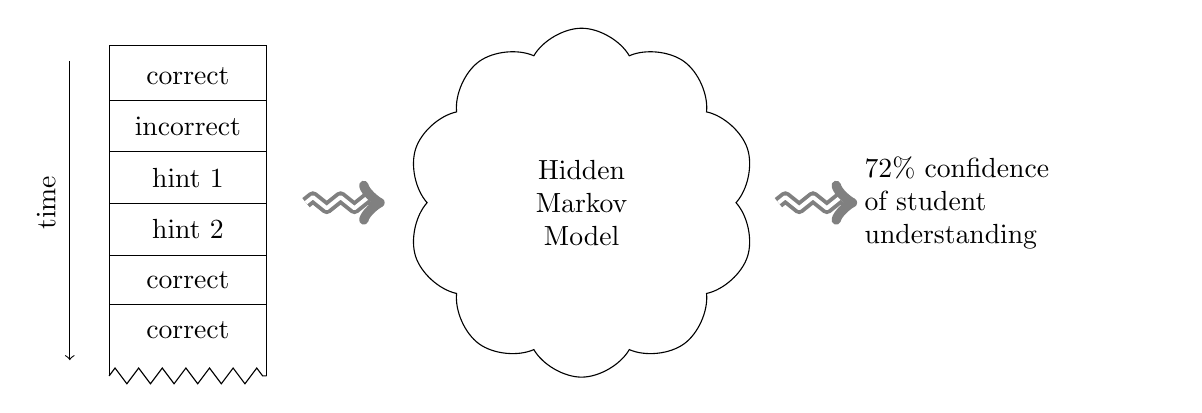
\begin{tikzpicture}[x=1cm,y=1cm]

\draw (-1,2) -- (1,2);
\draw (-1,2) -- (-1,-2.2);
\draw (1,2) -- (1,-2.2);

\draw [->] (-1.5,1.8) -- (-1.5,-2);

\node at (-1.8,0) [rotate=90] {time};

\draw [decorate, decoration={zigzag,segment length = 3mm, amplitude = 1mm}]  (-1,-2.2) -- (1,-2.2);

\node at (0,0) {\begin{minipage}{2cm}\begin{center}correct\\[.2cm] \hrule \vspace{.2cm} incorrect\\[.2cm] \hrule \vspace{.2cm} hint 1\\[.2cm] \hrule \vspace{.2cm}  hint 2 \\[.2cm] \hrule  \vspace{.2cm} correct\\[.2cm] \hrule \vspace{.2cm} correct \end{center}\end{minipage}};

\draw [->,gray, line join=round,line width=.5mm,double, double distance=.5mm,
decorate, decoration={
    zigzag,
    segment length=10,
    amplitude=2,post=lineto,
    post length=2pt
}]  (1.5,0) -- (2.5,0);

\node at (5,0) [cloud,draw,cloud puffs=10,cloud puff arc=120, aspect=1] {\begin{minipage}{1in}\begin{center}Hidden \\ Markov\\ Model\end{center}\end{minipage}};

\draw [->,gray, line join=round,line width=.5mm,double, double distance=.5mm,
decorate, decoration={
    zigzag,
    segment length=10,
    amplitude=2,post=lineto,
    post length=2pt
}]  (7.5,0) -- (8.5,0);

\node at (10.5,0) {\begin{minipage}{1.5in}72\% confidence \\ of student \\ understanding\end{minipage}};

\end{tikzpicture}}\end{center}
\end{frame}

\setbackgroundpictureblack{mooculus-screenshots/mooculus-exercise-index.png}
\begin{frame}
\end{frame}

\setdarkbackgroundpictureblack{mooculus-screenshots/mooculus-exercise-index.png}
\begin{frame}
  \Huge
  \begin{center}
    \color{white}
    Student works \\
    for mastery
  \end{center}
\end{frame}

\setdarkbackgroundpicturewhite{coursera-screenshots/coursera-quiz.png}
\begin{frame}[nofills]
\vfill
\begin{center}
\scaletowidth{\textwidth}{\huge\textsf{\textbf{\stacksame{Paper quizzes are all}{the same.}}}}
\end{center}
\vfill
\end{frame}

\setdarkbackgroundpictureblack{mooculus-screenshots/mooculus-exercise-index.png}
\begin{frame}
  \Huge
  \color{white}
  \begin{center}
    Massive, \\
    not mass-produced.
  \end{center}
\end{frame}

\settallbackgroundpicturewhite{photographs/Math_lecture_at_TKK.jpg}
\begin{frame}[label=classroom]
\end{frame}

\clearbackgroundpicture
\begin{frame}[nofills]
\Huge
%\Huge\textbf{What's the benefit?}

\vfill
\uncover<2->{\hfill\alt<1-2>{Cheaper?}{\textcolor{gray}{\sout{Cheaper?}}}%
\hfill\uncover<3->{\textcolor{red!50!black}{Better!}}\hfill\null}
\vfill
 
\end{frame}




%%%%%%%%%%%%%%%%%%%%%%%%%%%%%%%%%%%%%%%%%%%%%%%%%%%%%%%%%%%%%%%%
% PARTNERSHIPS
\clearbackgroundpicture
\againframe<9,10>{overview}

\clearbackgroundpicture
\begin{frame}[nofills]
\Huge\textbf{What's \textit{massive}?}

\vfill
\uncover<2->{\hfill\alt<1-2>{Enrollment?}{\textcolor{gray}{\sout{Enrollment?}}}%
\hfill\uncover<3->{\textcolor{red!50!black}{Data!}}\hfill\null}
\vfill
 
\end{frame}

\begin{frame}[nofills]
\huge
\vfill
\begin{center}
10.3 person--years
\end{center}
\vfill
\begin{center}
2,079,428 correct answers
\end{center}
\vfill
\end{frame}

\begin{frame}[nofills]
\scaletowidth{\textwidth}{\textbf{We now know priors.}}
\vfill
\huge
point plotting \hfill 91\% correct \\
trig derivatives \hfill 57\% correct \\
related rates \hfill 35\% correct \\
\vfill
\end{frame}



\begin{frame}[nofills]
\begin{center}
\includegraphics[height=0.9\textheight]{data/histogram-student-aces.pdf}
\end{center}
\end{frame}

\begin{frame}[nofills]
\begin{center}
\includegraphics[height=0.9\textheight]{data/exercise-odds-13.pdf}
\end{center}
\end{frame}

\begin{frame}[nofills]
\begin{center}
\includegraphics[height=0.9\textheight]{data/kaplan-meier-1.pdf}
\end{center}
\end{frame}

\begin{frame}[nofills]
\begin{center}
\includegraphics[height=0.9\textheight]{data/kaplan-meier-2.pdf}
\end{center}
\end{frame}

\begin{frame}[nofills]
  \huge
  \scaletowidth{\textwidth}{\textbf{Just-in-time tutoring}}

  \pause
  \vfill

  On a certain problem, \\
  95\% who answer correctly \\
  do so in 140 seconds.

  \pause
  \vfill

  Intervene then.

  \vfill
\end{frame}


%%%%%%%%%%%%%%%%%%%%%%%%%%%%%%%%%%%%%%%%%%%%%%%%%%%%%%%%%%%%%%%%
% PARTNERSHIPS
\clearbackgroundpicture
\againframe<10,11>{overview}

\clearbackgroundpicture
\begin{frame}[label=publish-teaching]
  \begin{tikzpicture}[remember picture,overlay]
    \only<2->{
      \node[xshift=-1.35in,yshift=0.25in] (top) at (current page.east) {\scaletowidth{0.4\textwidth}{\Huge\textbf{publish your}}};
      \node[xshift=-1.35in,yshift=-0.27in,anchor=base] (top) at (current page.east) {\scaletowidth{0.4\textwidth}{\Huge\textbf{teaching}}};
    }
  
    \only<1->{
      \node[xshift=1.35in,yshift=0.25in] (bottom) at (current page.west) {\scaletowidth{0.4\textwidth}{\Huge\textbf{publish your}}};
      \node[xshift=1.35in,yshift=-0.26in,anchor=base] (bottom) at (current page.west) {\scaletowidth{0.4\textwidth}{\Huge\textbf{research}}};
    }

    \only<3->{
      \node[yshift=0.75in,anchor=base] (underview) at (current page.south) {\scaletowidth{\textwidth}{``Fixed form'' makes discussion possible}};
    }
  \end{tikzpicture}
\end{frame}

\clearbackgroundpicture
%%%%%%%%%%%%%%%%%%%%%%%%%%%%%%%%%%%%%%%%%%%%%%%%%%%%%%%%%%%%%%%%
\begin{frame}[nofills,label=nsf-grant]%BADBAD
  \vfill
  \Large
  \begin{center}
    \stacksame{NSF TUES Grant}{\stacksame{\textbf{\stacksame{Interactive}{Textbooks}}}{Joint between Fowler, Snapp, Clemens}}
  \end{center}

  \vfill\pause

  \begin{center}
    \scaletowidth{\textwidth}{\stacksame{Open source platform for}{interactive textbooks.}}
  \end{center}

  \vfill
  \vfill
  \vfill
\end{frame}

%%%%%%%%%%%%%%%%%%%%%%%%%%%%%%%%%%%%%%%%%%%%%%%%%%%%%%%%%%%%%%%%
% PARTNERSHIPS
\clearbackgroundpicture
\againframe<11,12>{overview}

\settallbackgroundpicturewhite{github/sequences-and-series.png}
\begin{frame}
\end{frame}

\settallbackgroundpicturewhite{github/mooculus.png}
\begin{frame}
\end{frame}

\settalldarkbackgroundpicturewhite{github/mooculus.png}
\begin{frame}[nofills]
\vfill
\begin{center}
\Huge\textsf{\textbf{\scaletowidth{0.75\textwidth}{\stacksame{Version}{\stacksame{controlled}{repository}}}}}
\end{center}
\pause
\vfill
\begin{center}
\large\texttt{https://github.com/ASCTech/mooculus}
\end{center}
\vfill
\vfill
\end{frame}

\setbackgroundpicturewhite{mooculus-screenshots/mooculus-textbook-page.pdf}
\begin{frame}[nofills]
\end{frame}

\settallbackgroundpicturewhite{github/textbook-sample.png}
\begin{frame}
\end{frame}

\settalldarkbackgroundpicturewhite{github/textbook-sample.png}
\begin{frame}[nofills]
\vfill
\begin{center}
\Huge\textsf{\textbf{\scaletowidth{0.75\textwidth}{\stacksame{Anyone}{can edit}}}}
\end{center}
\vfill
\end{frame}

\settallbackgroundpicturewhite{github/commits.png}
\begin{frame}
\end{frame}

\settalldarkbackgroundpicturewhite{github/commits.png}
\begin{frame}[nofills]
\vfill
\begin{center}
\Huge\textsf{\textbf{\scaletowidth{0.75\textwidth}{\stacksame{History of}{changes}}}}
\end{center}
\vfill
\end{frame}

\settallbackgroundpicturewhite{github/contribution.png}
\begin{frame}[label=students-edit-1]
\end{frame}

\settalldarkbackgroundpicturewhite{github/contribution.png}
\begin{frame}[nofills,label=students-edit-2]
\vfill
\begin{center}
\Huge\textsf{\textbf{\scaletowidth{0.75\textwidth}{\stacksame{Students}{make edits}}}}
\end{center}
\vfill
\end{frame}

\clearbackgroundpicture
\againframe<12>{overview}

\settallbackgroundpicturewhite{github/contribution.png}
\begin{frame}[label=students-edit-1]
\end{frame}

\settalldarkbackgroundpicturewhite{github/contribution.png}
\begin{frame}<1-3>[nofills,label=students-edit-2]
\vfill
\scaletowidth{\textwidth}{\Huge\textsf{\stacksame{\textbf{\alert<2>{xMOOC}}}{\stacksame{merges with}{\textbf{\alert<3>{cMOOC}}}}}}
\vfill
\end{frame}

\clearbackgroundpicture
\againframe<13,14,15>{overview}

 %%%%%%%%%%%%%%%%%%%%%%%%%%%%%%%%%%%%%%%%%%%%%%%%%%%%%%%%%%%%%%%%
 \clearbackgroundpicture
 \begin{frame}[label=thanks,nofills]
   \vfill
   \begin{center}
   \Huge
    \scalebox{1.5}{\textbf{Thank You}}
   \end{center}
   \vfill
   \begin{center}
     \normalsize
   \begin{tabular}{lll}
   \textbf{Tom Evans:} & @taevans & \\
   \textbf{Jim Fowler:} & @kisonecat & http://kisonecat.com/
   \end{tabular}
   \end{center}
   \vfill
   \includegraphics[width=1in]{images/cc-logo.pdf}\hspace{0.5em}\footnotesize\scalebox{0.75}{\parbox[b]{4in}{except where otherwise noted on photographs,\\licensed for reuse under a Creative Commons BY-NC-SA License}}\hfill
   \null
   \vspace{12pt}
   \null
 \end{frame}

\end{document}
